\documentclass[12pt,]{article}
\usepackage{lmodern}
\usepackage{amssymb,amsmath}
\usepackage{ifxetex,ifluatex}
\usepackage{fixltx2e} % provides \textsubscript
\ifnum 0\ifxetex 1\fi\ifluatex 1\fi=0 % if pdftex
  \usepackage[T1]{fontenc}
  \usepackage[utf8]{inputenc}
\else % if luatex or xelatex
  \ifxetex
    \usepackage{mathspec}
  \else
    \usepackage{fontspec}
  \fi
  \defaultfontfeatures{Ligatures=TeX,Scale=MatchLowercase}
\fi
% use upquote if available, for straight quotes in verbatim environments
\IfFileExists{upquote.sty}{\usepackage{upquote}}{}
% use microtype if available
\IfFileExists{microtype.sty}{%
\usepackage{microtype}
\UseMicrotypeSet[protrusion]{basicmath} % disable protrusion for tt fonts
}{}
\usepackage[margin=1in]{geometry}
\usepackage{hyperref}
\hypersetup{unicode=true,
            pdftitle={Sending a Balloon to the Edge of Space},
            pdfauthor={Luker Bowsher, John Kim, Vivian Liu, Simon Oros, Caroline Pang, Alec Vercruysse},
            pdfborder={0 0 0},
            breaklinks=true}
\urlstyle{same}  % don't use monospace font for urls
\usepackage{longtable,booktabs}
\usepackage{graphicx,grffile}
\makeatletter
\def\maxwidth{\ifdim\Gin@nat@width>\linewidth\linewidth\else\Gin@nat@width\fi}
\def\maxheight{\ifdim\Gin@nat@height>\textheight\textheight\else\Gin@nat@height\fi}
\makeatother
% Scale images if necessary, so that they will not overflow the page
% margins by default, and it is still possible to overwrite the defaults
% using explicit options in \includegraphics[width, height, ...]{}
\setkeys{Gin}{width=\maxwidth,height=\maxheight,keepaspectratio}
\usepackage[normalem]{ulem}
% avoid problems with \sout in headers with hyperref:
\pdfstringdefDisableCommands{\renewcommand{\sout}{}}
\setlength{\emergencystretch}{3em}  % prevent overfull lines
\providecommand{\tightlist}{%
  \setlength{\itemsep}{0pt}\setlength{\parskip}{0pt}}
\setcounter{secnumdepth}{5}
% Redefines (sub)paragraphs to behave more like sections
\ifx\paragraph\undefined\else
\let\oldparagraph\paragraph
\renewcommand{\paragraph}[1]{\oldparagraph{#1}\mbox{}}
\fi
\ifx\subparagraph\undefined\else
\let\oldsubparagraph\subparagraph
\renewcommand{\subparagraph}[1]{\oldsubparagraph{#1}\mbox{}}
\fi

%%% Use protect on footnotes to avoid problems with footnotes in titles
\let\rmarkdownfootnote\footnote%
\def\footnote{\protect\rmarkdownfootnote}

%%% Change title format to be more compact
\usepackage{titling}

% Create subtitle command for use in maketitle
\newcommand{\subtitle}[1]{
  \posttitle{
    \begin{center}\large#1\end{center}
    }
}

\setlength{\droptitle}{-2em}

  \title{Sending a Balloon to the Edge of Space}
    \pretitle{\vspace{\droptitle}\centering\huge}
  \posttitle{\par}
    \author{Luker Bowsher, John Kim, Vivian Liu, Simon Oros, Caroline Pang, Alec
Vercruysse}
    \preauthor{\centering\large\emph}
  \postauthor{\par}
      \predate{\centering\large\emph}
  \postdate{\par}
    \date{November 13, 2018}

\usepackage{setspace}
\usepackage{gensymb}

\begin{document}
\maketitle
\begin{abstract}
This paper details 6thsense, a mission to send a weather balloon to to
edge of space in order to study Earth's atmosphere. The weather balloon
is outfitted with a payload that includes a camera, inside and outside
temperature sensors, a barometer, multiple GPS tracking devices, as well
as a host of individual experiments. The balloon most likely reached an
altitude of 20,000 meters, into the stratosphere and ozone layer. The
balloon was successfully recovered after approximately one and a half
hours of flight.
\end{abstract}

\newpage

\setcounter{secnumdepth}{2} \setcounter{tocdepth}{2} \tableofcontents
\newpage
\onehalfspacing

\section{Introduction}\label{introduction}

There are four main layers to the atmosphere: the troposphere,
stratosphere, mesosphere, and thermosphere. The \textbf{troposphere} is
the section of the atmosphere from roughly 0km to 15km, and is the layer
in which we live. It includes 75\% of the mass of all gases in the
atmosphere, consisting of 78\% nitrogen gas, 21\% oxygen, and less than
1\% of argon, carbon dioxide, and other constituents. Because it is both
the lowest in altitude and most massive layer, the pressure in the
troposphere is the greatest: 100kPa. As you increase altitude in the
troposphere, temperature decreases to about -60C. The
\textbf{stratosphere} is the section from roughly 15km to 50km. The
ozone layer, or the region in the atmosphere which absorbs most UV rays,
is within the stratosphere at about 20km in altitude. The pressure in
the stratosphere is 10kPa. The \textbf{mesosphere} is the region from
50km to 80km. The pressure in the mesosphere is 0.1 kPa. Finally, the
\textbf{thermosphere} is the highest in altitude of the four layers,
spanning from 80km into outer space. Here, the pressure is only 0.01kPa,
as it is the least dense of the layers. The few air molecules in the
thermosphere are heated to extremely high temperatures by the Sun's
radiation. However, because there are so few molecules, we cannot
measure an appreciable difference in overall temperature, so the
effective temperature of the thermosphere is less than that of the
mesosphere.

The layers relevant to our experiment are the troposphere and
stratosphere, as our balloon launch was designed to reach a maximum
altitude of 30km (about the middle of the stratosphere but past the
ozone layer). Therefore, we had to prepare the payload for temperatures
as low as -60C and pressure as low as 10kPa (in the stratosphere). We
expect to encounter the lowest temperature in the troposphere, around an
altitude of 10km. As the balloon rises from sea level to the top of the
troposphere, we expect to see temperature decrease because the ground
absorbs most of the sun's radiation (as opposed to the gas particles).
However, as the balloon enters the stratosphere, we expect an increase
in temperature due to the ozone layer's blockage of UV rays. The UV rays
that the ozone layer absorbs causes the gas particles in the
stratosphere to heat up, so temperature increases with altitude. As the
balloon gains altitude, the density of air around it decreases, so the
pressure decreases.

The presence of greenhouse gasses in the atmosphere contribute to the
warming of the earth's surface and the troposphere because of the
greenhouse effect. The greenhouse effect describes the trapping of heat
within the earth's atmosphere via the infrared absorption of certain
molecules.

When infrared radiation enters the atmosphere, short-wave infrared
radiation (700 - 1000 nm) does not effectively interact with greenhouse
gasses. The photons instead pass through the atmosphere and reach the
surface of the earth. Here, they are absorbed by the surface of the
earth and get reemitted as a lower energy, longer-waved infrared photon.
Greenhouse gasses can now absorb these lower energy photons and reemit
them. This absorption and reemission warms the troposphere by increasing
the kinetic energy the atmosphere. Additionally, greenhouse gasses can
reemit photons back towards the surface of the earth, increasing the
temperature of the earth's surface. By impeding the tendency for
long-wave radiation to leave the atmosphere, the greenhouse effect
increase the temperature of the troposphere and surface.

The spectroscopy that explains the greenhouse effect concerns molecular
vibration. Infrared photons excite vibrations in molecules. Since the
vibrational frequency of atoms are quantized, only certain energies will
excite vibration in a molecule. Different molecules can exhibit
different vibrational modes. A molecule with more atoms has more
vibrational modes. The infrared selection rule states that a vibrational
mode is active when it is changing the dipole moment of the molecule. An
active vibrational mode is a molecular vibration that can be excited by
an infrared photon. Thus, infrared photons will only be absorbed when
that molecule's dipole moment is changing. Molecules such as nitrogen
and oxygen will never exhibit a change in their dipole moment due to
vibration because their only vibrational mode involves the singular
oscillation of the distance between two atoms. Thus, they cannot absorb
infrared radiation in order to partake in the greenhouse effect and are
not considered greenhouse gasses. R On the other hand, many atmospheric
molecules that have more than two atoms have more complex vibrational
modes. These active vibrational mode gasses, such as nitrogen dioxide
and water, are called greenhouse gasses.

As the greenhouse effect warms the planet, many factors accelerate the
temperature rise by creating positive feedback loops. Positive feedback
loops amplify any global increase in temperature. One positive feedback
loops is created when rising temperatures melt glaciers. These white and
reflective icy surfaces melt into dark oceans which absorb more
radiation and heat up faster. This explains the approaching transition
from a permanent to a seasonal ice cover in the Arctic Ocean. Thus
temperature increases accelerate.\footnote{\url{https://www.nature.com/articles/s41598-017-08467-z}}
Another positive feedback loops involves the melting of permafrost. A
quarter of the northern hemisphere is covered in permafrost that holds
concentrated methane and carbon dioxide. Slight growths in temperature
are enough to thaw the permafrost. When it melts, these greenhouse
gasses are released into the atmosphere. Thus, the greenhouse effect
amplifies and global temperature growth accelerates. \footnote{\url{http://science.sciencemag.org/content/340/6129/183}}
Finally, humidity is also a positive feedback loop. As global
temperatures rise, the atmosphere can hold more water vapor because less
of it gets condensed. Water vapor is a greenhouse gas itself. Thus any
increase in global temperatures will be amplified due to the water vapor
positive feedback loop.

The annual increase of atmospheric carbon dioxide concentration is
approximately 100 times greater in the past 60 years than it has been
during any previous natural increase.F Additionally, methane
concentrations have more than doubled since the start of the industrial
revolution.B Partly due to the increase of these gas concentration along
with many positive feedback loops, the planet's average surface
temperature has risen 0.9\degree C since the late 19th century.F With
rising temperatures comes the consequences of severe weather patterns,
flooding and other natural disasters. Collecting atmospheric data of
things such as temperature and gas concentrations informs our
understanding of the progression of the greenhouse effect. With this
information, we can begin to look at ways to impede rising global
temperatures.

The Panel on Climate Change has recognized that as global temperatures
rise, lightning strikes will occur more frequently. As our skyscrapers
get higher and multiply, lightning strike sourced Terrestrial Gamma ray
Flashes (TGF) become a concern.

TGFs are short, powerful bursts of gamma rays detected in the
atmosphere. Each burst contains 10\^{}17 to 10\^{}19 gamma rays and last
about 1 ms. They were first detected in the 1950s. The United States,
concerned with the Soviet Union's nuclear progress used satellites to
detect gamma rays and track the enemy's progress. After observing long,
5-10 second gamma ray glows (suspected to be Gamma ray Bursts (GRB) from
stars), the U.S. sent more satellites to explore GRB further. In
addition to detecting GRB, the data from these satellites led to the
discovery of TGFs. When short, gamma ray bursts were analyzed for their
source locations, researchers noticed that these burst mainly came from
coastal sites on the equator. After recognizing a correlation with
lightning prone areas and these short gamma ray bursts, C. T. R.
Wilson's theory concerning a Relativistic Runaway Electron Avalanche
(RREA) was applied to discover TGFs.

Wilson's RREA theory relies on a quantum properties of electrons. As the
velocity of normal objects traveling through the atmosphere increases,
the air resistance increases also. Therefore, in a constant force field,
the object will reach a terminal velocity. For electrons however, while
the air resistance initially increase with its speed, at high
velocities, the air resistance on the electron begins to decrease. This
is because at relativistic speeds, the electron can avoid interactions
with other molecules. Thus, after the electron reaches a certain speed,
it will never reach a terminal velocity and accelerate indefinitely as
long as it is still in a force field. Electrons that escape terminal
velocity are called runaway electrons. The second part of Wilson theory
involves an explanation of the ``Avalanche.'' Runaway electrons can
knock other electrons while accelerating and cause them to become
runaway electrons also. This creates an exponential increase of runaway
electrons as more and more electrons interact.

The RREA theory explains a hypothesis for TGFs. The field that
accelerates runaway electrons is an electric field produced by the
separation of charges in thunderclouds. The energy field required to
cause a RREA is powerful enough to cause lightning strikes. Thus, the
occurrence of a lightning strike is correlated with that of a TGF. As
electrons accelerate through the atmosphere, they can undergo
Bremsstrahlung interactions with the nucleuses of air molecules. When an
electron is deflected around a nucleus, a powerful Bremsstrahlung photon
is emitted. Since an avalanche of electrons undergo this interaction,
this explains the massive quantity of gamma rays contained in one TGF.

While there is an abundance of research done on upward directed TGFs
(those detected by the satellites in the 1950s), there is a lack of data
detecting downward directed TGFs. Currently, researchers led by David M.
Smith at UC Santa Cruz and other researchers around the world are using
a multitude of methods to detect downwards directed TGFs. Some methods
include sending detectors in cargo planes, on weather balloons and on
the ground in thunder prone areas. Since TGFs are so powerful, detectors
usually fail if they are near a TGF because of the sheer amount of
energy exerted. This field of research is relatively new and active.

\textbf{INSERT PRESSURE MODEL ANALYSIS HERE}

The exponential model for temperature vs altitude, where altitude is
less than 11km (or where altitude is within the troposphere) is:
T=T0(1-h/44329), where h=height in meters, and T0=temperature at sea
level. This relationship shows a negative relationship between height
and temperature. As altitude increases within the troposphere,
temperature decreases.

\section{Experiments Conducted}\label{experiments-conducted}

The payload included two tracking devices, a GoPro Hero 3+ to record the
ascent, and sensors to monitor the atmosphere and record altitude data.
In addition, each team member implemented a sensor as part of an
individual experiment. This paper focuses on the results of the group
experiments, but the setups for the individual experiments are still
described. Separate papers can be found for each team member's
individual experiment.

\subsection{Group Experiments}\label{group-experiments}

\begin{longtable}[]{@{}lll@{}}
\toprule
Sensor & Function & Model\tabularnewline
\midrule
\endhead
Real Time Clock & Accurate Timing & Sparkfun DS1307 RTC\tabularnewline
GPS & Location Data & Sparkfun Venus GPS\tabularnewline
Barometer & Altitude Data & Vernier Gas Pressure Sensor\tabularnewline
Temperature & Outside Temperature & Adafruit BME280\tabularnewline
Humidity & Outside Humidity & Adafruit BME280\tabularnewline
Temperature & Inside Temperature & Thermistor\tabularnewline
\bottomrule
\end{longtable}

In addition, a PicoAPRS was used to provide live GPS coordinates,
altitude, heading, and speed measurements.

These sensors were picked in order to be able to track the balloon
through its flight and provide baseline measurements to compare other
individual sensors to. By recording accurate altitude and time
measurements with the measurement of every other sensor, sensor data can
be analyzed with respect to both time and altitude. Furthermore,
recording temperature data for both inside and outside the payload helps
provide diagnostic data for if any specific part of the payload fails,
and provides another baseline to compare any other sensor measurements
to. The Humidity sensor not only provides humidity data which can be
analyzed with respect to Altitude, but it can also determine when the
payload is in a cloud, which could affect the measurements of other
sensors.

\subsection{Individual Experiments
Conducted}\label{individual-experiments-conducted}

\begin{longtable}[]{@{}ll@{}}
\toprule
Team.Member & Experiment\tabularnewline
\midrule
\endhead
Alec Vercruysse & Spectrometer\tabularnewline
Luke Bowsher & Accelerometer\tabularnewline
Simon Oros & \sout{Geiger Counter}*\tabularnewline
Vivian Liu & Light Intensity Sensors\tabularnewline
Caroline Pang & UVB Sensor\tabularnewline
John Kim & Methane Sensor\tabularnewline
\bottomrule
\end{longtable}

*shortly before launch it was discovered that the Geiger Counter was
non-operable and therefore it was taken out of the payload. Instead,
Simon Oros focused on \_\_\_\_.

\textbf{INCLUDE INDIVIDUAL MOTIVATIONS HERE}

\section{Physical Design}\label{physical-design}

lorem ipsum

\section{Cut Down Mechanism}\label{cut-down-mechanism}

lorem ipsum

\section{Electrical and Software
Design}\label{electrical-and-software-design}

lorem ipsum

\section{Tracking The Payload}\label{tracking-the-payload}

One of the largest priorities was tracking the balloon to ensure a
successful recovery. To do this, two completely independent tracking
systems were implemented to add redundancy and mitigate the chances of
completely losing the payload upon landing. The first method was a
pre-built PicoAPRS transceiver, a small separately powered 144.39 MHz
transceiver that utilizes an amateur radio network to broadcast location
details that can be accessed through a website. The backup system was
transmitting location data obtained by a Venus GPS module through a
line-of-site, point to point, 900Mhz receiver, with a novel protocol
developed with an emphasis on simplicity of parsing even broken packets.
Lastly, to narrow down the location of the payload once it touched down,
a separate transmitter at 147.065 MHz was included to use for
fox-hunting upon touchdown.

\subsection{The Global Positioning
System}\label{the-global-positioning-system}

The Global Positioning System (GPS) is a system of satellites in Medium
Earth Orbit around Earth which provide accurate location details to any
device connecting to the network. The orbits of these 27 satellites,
while not geostationary, ensure that four satellites are visible from
any location on Earth at any given moment.\footnote{\url{http://www.astronomy.ohio-state.edu/~pogge/Ast162/Unit5/gps.html\#note01}}
By evaluating the time taken for GPS signals to be sent down to earth in
the form of radio waves traveling at the speed of light, a GPS receiver
is able to calculate the distance between it and the satellite. Using
this distance information gained from at least three satellites, a GPS
receiver is then able to ``trilaterate'' to find its location relative
to the satellites.\footnote{\url{http://www.physics.org/article-questions.asp?id=55}}
Given the distance between a satellite, a GPS unit must be located on a
sphere extending outward with a radius of that distance. With
information from three satellites, three spheres are given, and
generally the intersection of three spheres results in two points, once
which can be discarded due to the fact that it would not be physically
possible for the GPS receiver to be located there.

The Department of Commerce has placed regulations on exports that could
potentially threaten the United States. This includes GPS receivers that
can provide data when they are above 18,000 meters or their speed is
above 1000 knots, due to their potential use in Intercontinental
Ballistic Missiles.\footnote{\url{http://ravtrack.com/GPStracking/cocom-gps-tracking-limits/469/}}Some
manufacturers have implemented these limits by shutting down the system
when either condition is met, and some manufacturers have implemented
these limits by shutting down the system only if both conditions are
met. This is an important distinction, since high altitude balloons
often exceed the height limit of 18,000 meters. Sparkfun's Venus GPS
module, which uses the Venus634FLPx GPS chipset, is known to allow
altitudes of over 18,000 meters, given that the speed of the GPS
receiver is not calculated to be more than 1000 knots.\footnote{\url{https://ukhas.org.uk/guides:gps_modules}}

\subsection{The PicoAPRS Transceiver}\label{the-picoaprs-transceiver}

The primary tracking system onboard the balloon was a PicoAPRS,
developed by Taner Schenker (DB1NTO). This is a small transceiver that
can receive and broadcast on the Automatic Packet Reporting System
(APRS). Most importantly, it contains its own separate GPS chip that
allows it to broadcast its location to the APRS network. This device is
completely self contained, including its own 850MAh Lithium Ion battery,
making it a perfect candidate for tracking -- even if all other systems
on the balloon have failed, the PicoAPRS should still be able to
transmit its location. Furthermore, the PicoAPRS provides a simple menu
for device configuration, to enable the performance desired.
Specifically, the PicoAPRS transmitted GPS beacons at a power of 1 Watt
over intervals of 60 seconds. The PicoAPRS did this with Menlo School's
callsign, N6MLO, and a unique SSID, 9, that differentiated the packets
sent by 6thsense's PicoAPRS from other concurrent Menlo School balloon
launches.

\subsection{The APRS Network and
MIC-Encoding}\label{the-aprs-network-and-mic-encoding}

A very important benefit of using the PicoAPRS is that it uses the
Automatic Packet Reporting System (APRS). This amateur radio network,
developed by Bob Bruninga (WB4APR) uses digipeaters to forward properly
formatted broadcasted beacon packets to other stations in the area to
effectively extend the range of a single transmitter. Rather than
focusing on ensuring that a packet is received by all digipeaters, this
protocol focuses on redundancy through packet ``multiplication'' by
having each digipeater that receives the signal propagate it outward
through the network. While the exact details of how many ``hops'' a
packet can take through the network before transmission ends are
dependent on the settings present in the header of the packet. This
system became popular, especially for transmitting GPS data and tracking
vehicles, and eventually specifications were developed to transfer
packet data to the web through APRS-Internet Service
(APRS-IS).\footnote{\url{http://www.aprs-is.net/}} The aprs.fi website,
which interfaces with APRS-IS and displays live telemetry data
superimposed on google maps, provided a simple method of tracking the
balloon during the launch.

The APRS network transmits packets through a single AX.25 data link
protocol, which specifies the structure of frames to be sent through the
network. Specifically, it uses Unnumbered Information (UI) frames, a
type of AX.25 frame that is transmitted without any expectation of a
response confirming reception, and reception is not guaranteed. APRS
supports different encoding of these AX.25 UI-frames, however, to allow
for different uses of the network. The PicoAPRS transmitter uses
``Mic-Encoding'' (MIC-E), a method that allows for extremely compressed
packets that still contain position, course, speed, a message, and all
relevant path settings and necessary headers. This achieved by writing
compressed latitude information in the destination address field of the
AX.25 frame, and compressed Longitude information in the frame's
Information Field. By transmitting extremely short packets that are
still supported by the APRS network and aprs.fi, Mic-E can improve the
reliability of the beacons transmitted.

APRS is transmitted using Frequency Modulated signal at 144.39 MHz.
Frequency Modulation works by altering the frequency of a carrier wave
to encode information.

The PicoAPRS was chosen because the system had worked historically for
past ASR Balloon Launches. During testing, however, the APRS network
often failed to receive beacons, due to the fact that most tests were
conducted at ground level, where line of sight to repeater stations was
often not available. Furthermore, there was no method of testing the
maximum altitude that beacons could be sent from before connection to
the APRS network was lost. Lastly, since Lithium-Ion batteries are known
to work poorly in below freezing temperatures, there were concerns that
the unit might shut down once the temperature dropped, if not properly
insulated. Due to these concerns, a backup tracking system was developed
that did not rely on the PicoAPRS and APRS network should the PicoAPRS
unit fail.

\subsection{The 900MHz Venus GPS
Transciever}\label{the-900mhz-venus-gps-transciever}

The backup tracking system involved sending GPS along with other
telemetry data from the main arduino mega to the base station using
Digikey 9XTend 900MHz transceivers.\footnote{\url{https://www.sparkfun.com/datasheets/Wireless/Zigbee/xtend-productmanual.pdf}}
The use of these transceivers provided a high power 1 Watt signal in a
relatively clear band that let a novel communications protocol be
implemented that allowed for ease of parsing. The 9XTend module
interfaced easily with both balloon and base station arduinos through
Universal Asynchronous Receiver-Transmitter (UART) Serial. Since the
Arduino Mega provides three usable Serial ports, one was used to send
data to the 9XTend Module. By taking advantage of Arduino's Serial
library, a library was developed that allowed the 9XTend modules to
transmit ASCII encoded bytes, which, given some stream editing by the
base station to remove ASCII control characters injected by the base
9XTend Module, is parsable as an ASCII byte stream by software on the
base station.

\subsubsection{A Novel Transmission
Protocol}\label{a-novel-transmission-protocol}

To send readable GPS and telemetry data to the base station, a simple
multi-layer protocol was implemented with design considerations in mind
to allow for simple parsing and data analysis, simple manual error
detection, no error correction or discarding of broken transmissions, no
set packet size, zero unnecessary headers or other packet configuration
information, and no transmitter handshaking requirements. This allows
for simplex communication between the payload and base station. This
also ensures that all bytes that are received by the 9XTend, which
implements a Cyclic Redundancy Check on every byte received to ensure
its value is correct, are sent to the base station software for parsing.
Note that the 9XTend module not protect against lost bytes, so packets
could often be broken or missing some information. Through this new
protocol, no partially broken packets would be lost or deleted if the
signal was weak. Since the 9XTend Module transmitted all data for
sensors connected to the arduino as a redundancy in case the payload was
not retrieved or there was a problem logging data to the onboard SD
card, it is also crucial to be able to differentiate between two
different values in a partially broken packet.

A protocol was used with the following form to transmit n values:

\texttt{******\textless{}value-1\textgreater{}-\/-\/-\/-\/-\/-\textless{}value-2\textgreater{}-\/-\/-\/-\/-\/-...-\/-\/-\/-\/-\/-\textless{}value-n\textgreater{}}

Where \texttt{\textless{}value-i\textgreater{}} is an ASCII encoded,
calibrated and human readable sensor value. This allows for simplex
operation in which a base station can tune in at any time--if the base
station loses reception or power for some reason, it can listen in for
the next packet when it comes back online by simply waiting for the 6
stars indicating the start of a packet. Furthermore, data was encoded in
ASCII bytes to let the output be human readable with little computation.
This way, the output stream could be easily analyzed without having to
convert bytes containing raw numerical values into ASCII text. This gets
rid of the need to make specifications for negative numbers and floats,
and the need to specify the size of transmitted data. By encoding each
digit as an ASCII byte, it was simple to account for negative numbers by
preceding the value with a dash just as is normally done with displayed
numbers, and to account for floats by adding a decimal place behind the
ones digit. Furthermore, more complicated sensor readings like GPS and
Spectrometer output that contained ASCII formatted text could be sent
as-is with zero need for manipulation. Since 12 values were transmitted
(refer to Section 5) with uncompressed ASCII bytes, packet sizes were
long: up to 240 bytes. Because of this, there were often small failures
in the packet were a byte or series of bytes was not received. Such
packets were still logged with the notion that it was still possible to
extract most of the data out of them instead of having them completely
go to waste. To ensure that the start of a packet could be recognized
and separate values could be delineated properly, however, a full six
bytes was used to mark the beginning of a transmission, and breaks
separating values. This data was only transmitted about once every 12
seconds, partly to serve as flow control in order to not overload the
transmitter's buffer, and partly to conserve battery power, as the
9XTend module consumed 1 Watt while transmitting and was connected to
the same battery as the Arduino Mega running all the sensors and SD
logger.

\subsubsection{Physical Considerations and Antenna
Design}\label{physical-considerations-and-antenna-design}

Since the 9XTend module transmits directly to the base station, line of
sight was crucial to maintain connectivity. An omnidirectional whip
antenna had to be used on the balloon module since the heading and
position relative to the base station was constantly changing and
therefore the transmissions could not be directed in one particular
direction. While it might have been possible to use a directional
antenna at the base station to increase signal, it was not ideal since
the balloon was followed in a chase van, and directing an antenna
outside the van would be imprecise and lead to a lossy connection.
Furthermore, 900MHz yagi antennas are not readily available in stores
and time was not properly budgeted to assemble and test one by hand.
Therefore, a 900Mhz whip antenna was mounted to the top of the chase van
to connect to the receiving 9XTend Module.

\subsection{Fox-Hunting with a 147.065MHz
Transmitter}\label{fox-hunting-with-a-147.065mhz-transmitter}

While GPS modules, if they have signal at ground level, are usually able
to report location down to a few feet, the PicoAPRS was only expected to
be able to connect to the APRS network at a few thousand feet before it
lost line of sight to repeater stations, and there was no expectation to
receive signal from the 900MHz point to point transmitter, which also
relied on line of sight, which would not be available when the payload
had touched down. Therefore, it was expected that the latitude and
longitude data provided by both the PicoAPRS and the 9XTend modules
would be too imprecise to be able to locate and retrieve the payload. To
further narrow down the location of the module, a 147.065MHz transmitter
was included that broadcasted a distinct audio beacon along with Menlo
School's callsign in morse code, every minute. This enabled the use of
Fox-Hunting techniques to recover the payload once the tracking team was
in range of the beacon.

By having an omnidirectional whip antenna transmit the beacon and a
directional yagi antenna receive the beacon, the direction of the
balloon relative to the fox-hunt receiver was able to be calculated once
the fox-hunt receiver was in range of the beacon. Since directional
antennas receive greater power in the direction they're pointed, by
identifying in which direction the antenna receives the strongest
signal, it is possible to identify the source of the beacon and move in
that direction until the payload is found.

\subsubsection{Fox-Hunting Yagi Antenna
Design}\label{fox-hunting-yagi-antenna-design}

\textbf{CAROLINE STILL NEEDS TO WRITE}

\subsubsection{Determining Signal Strength with a Variable RF
Attenuator}\label{determining-signal-strength-with-a-variable-rf-attenuator}

A crucial component of Fox-Hunting is measuring the received signal
strength. Since the transmitter transmits an audio signal, one can
simply listen to the clarity of the received audio to do so. If the
receiver is close to the transmitter, however, and the received signal
is very strong, in tests it was hard to differentiate between a weak and
a strong signal and narrow down on the proper direction. To be able to
better distinguish signal strength, a variable Radio Frequency (RF)
attenuator was used to lower the strength of the signal until distortion
in the audio could clearly be heard, and therefore it was easier to
determine whether the signal strength improved or decreased after a
change in direction of the antenna.

The RF Attenuator used to lower the received signal mixes a constant
4MHz with the received signal in order generate two sidebands 4MHz above
and below the base signal. This sideband is an attenuated version of the
original signal, and tuning the receiving radio to the base frequency
plus 4 MHz, 151.065MHz, lets one monitor this attenuated signal.
Furthermore, the amplitude of the 4 Mhz signal can be varied in order to
vary the strength of the sideband, effectively providing varied
attenuation.

\subsection{Results}\label{results}

The balloon powered on at precisely 1:00pm with all three systems
working: location information showed up on aprs.fi, the base station
received transmissions including GPS information, and the HAM radio used
for fox-hunting received 6thsense's unique tone.

\subsubsection{The Venus GPS and 9XTend
Module}\label{the-venus-gps-and-9xtend-module}

Only about 14 minutes later, however, once the balloon had reached
approximately 2600 meters, the Venus GPS module lost reception and
stopped transmitting latitude and longitude data. The 9XTend module
continued to transmit other telemetry data including altitude, however,
for the duration of the flight, until the payload touched down, in which
most likely the crash disconnected some circuitry essential to
transmission, or the batteries lost their charge. Once the payload
reached approximately 7800 meters, 9XTend transmissions became
significantly damaged to the point where the data could no longer be
programmatically parsed by simply finding values between the delimiters
specified. Packets continued to be somewhat recognizable up to 20,000
meters, the estimated maximum height the ballon reached at approximately
1:50pm. Shortly after, at 1:53pm, the first packet was received
indicating the balloon had began a slow descent (see Section 4). During
descent, especially back at around 7800 meters, transmissions became
more recognizable but still required manual interpretation. Transmission
stopped after around 7400 meters, indicating that most likely the
arduino lost power at 2:17pm, two and a quarter hours after powering up.

Unfortunately, while the 9Xtend module paired with the Venus GPS failed
its primary mission of providing GPS information, the transmission
system worked very well for the entirety of the time that it was
powered. Not only did it provide the base station with live altitude
data, it transmitted sensor data, including that of individual
experiments. This proved invaluable to the team, since the SD logging
module failed to write data.

Since the Venus GPS receiver was mounted at the top of the payload, with
its line of sight to the GPS satellites obstructed by only the balloon,
and the GPS chips did not have the 18,000 meter limit, there is no clear
reason for why the system failed. One possibility is that the outside
temperature of 16 degrees Celsius was too low for the circuitry
involved. Another is simply that the antenna was somehow internally
damaged or not optimal. Upon touchdown, all GPS wiring was still in
place, indicating that it was not an issue with the circuit or placement
of the antenna.

The last possible reason is that other circuitry such as the arduino
microprocessor in the payload generated radio frequency interference.
The GPS center frequency is 1575.42MHz, however, and the crystal
oscillator providing the clock for the Arduino Mega only runs at 16MHz,
which indicates that other circuits in the payload were most likely not
causing this issue.

\subsubsection{The PicoAPRS and APRS
Network}\label{the-picoaprs-and-aprs-network}

The PicoAPRS consistently broadcasted packets that were picked up by the
network up to almost exactly 10,000 meters at 1:30pm, before the network
lost reception. The PicoAPRS continued transmitting accurate location
data, however, and the network once again started receiving
transmissions at 2:16pm, once the payload had fallen to approximately
8200 meters. The final transmission came at 2:36pm just 250 meters above
the ground. Overall, this system worked flawlessly to provide accurate
location data while in range of the network, between approximately 250
meters and 9000 meters in altitude. Fortunately, the insulation added to
the payload was able to keep its Lithium Ion battery warm enough to
maintain power. Since the Venus GPS failed early into the flight,
tracking the payload relied on the APRS for accurate location data until
the chase van got in range of the fox-hunt beacon .

\subsubsection{The Fox-Hunt Beacon and Yagi
Antenna}\label{the-fox-hunt-beacon-and-yagi-antenna}

The final PicoAPRS beacon came from a very low altitude, narrowing down
the final location to a radius of less than 200 meters. Once the chase
van arrived at the location described by the final APRS packet, the team
was immediately able to pick up the Fox-Hunt signal even with the
attenuator attached. A single sweep of the Yagi antenna revealed the
payload was due South along the road, and the payload was found less
than 50 meters away from the road, lying hidden from view of the road on
a small hill. The antenna, attenuator, transmitter and receiver all
worked flawlessly to lead to a simple recovery in the time it took to
walk from the parked van to the touchdown point of the payload.

\section{Sensor Calibration}\label{sensor-calibration}

To ensure that the payload would collect accurate and reliable data, the
lightweight sensors used and controlled by the Arduino board were
thoroughly calibrated. The three group sensors calibrated were the
temperature and humidity sensors onboard the Vernier Gas Pressure
Sensor, and the Vernier Gas Pressure Sensor. The outputs of all three
sensors were compared to standards, which were already known to be
reliable and accurate. The standards, despite their accuracy, could not
be used in the payload because of their heavy weight and large size,
hence it was crucial that the small and light Vernier and BME280 sensors
were calibrated.

\subsection{The Vernier Gas Pressure
Sensor}\label{the-vernier-gas-pressure-sensor}

The Vernier Gas Pressure Sensor, model GPS-BTA, was calibrated to the
Extech SD700 Barometric Pressure/Humidity/Temperature Datalogger, which
was used as our standard for pressure. The Vernier sensor was connected
to an Arduino microcontroller with a Vernier Analog Protoboard Adaptor
and configured to log data onto a micro-SD card every 1.50 seconds.
Instead of having a output unit of hPa or kPa, the Arduino maps input
voltages between 0 to 5 volts to 10-bit integer values between 0 and
1023---a total of 1024 bins with 0.49 mV resolution. Thus, each unit
represents 4.9 mV. The SD700 has a pressure range of 10 to 1100 hPa,
fine resolution of 0.1 hPa, optimal temperature range of 0 to 50°C,
response time of 10 milliseconds, and total accuracy with its factory
calibration ±4 kPa. It requires 6 AAA batteries, and records data to an
external SD card in the format of an Excel worksheet. It was configured
so that it sampled data every five seconds to have smoother and more
gradual changes in pressure. After both sensors were turned on at the
same time to easily compare the data later, they were immediately placed
in a vacuum chamber, in which air and other gasses are removed by a
vacuum pump, thus creating a low-pressure environment inside the
chamber. The release valve was closed and the vacuum pump was opened.
When the pressure reading from the valve reached its minimum of
approximately 0 hPa, the vacuum pump was then disconnected. An important
part of the pressure calibration process was having ``plateaus,'' or
multiple data points at various pressure levels. To have plateaus in the
data, the release valve was slowly opened and closed right after, and
this process was repeated after waiting approximately 45 seconds
multiple times. Graph 5 and 6 show the varying pressure readings from
the standard Extech sensor and Arduino Vernier sensor across time,
respectively.

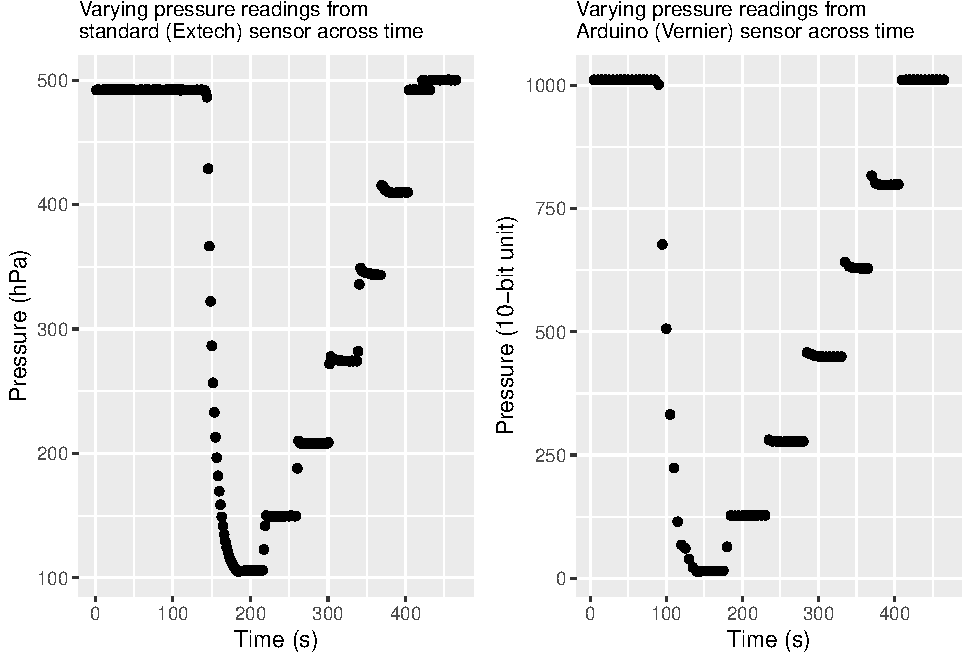
\includegraphics{paper_files/figure-latex/vernier_calibration-1.pdf}

Graph 7, shown below, shows the conversion between the output of the
standard (Extech) sensor and that of the Arduino (Vernier) sensor,
including the equation to convert the Arduino's 0.49 mV resolution units
to kPa.

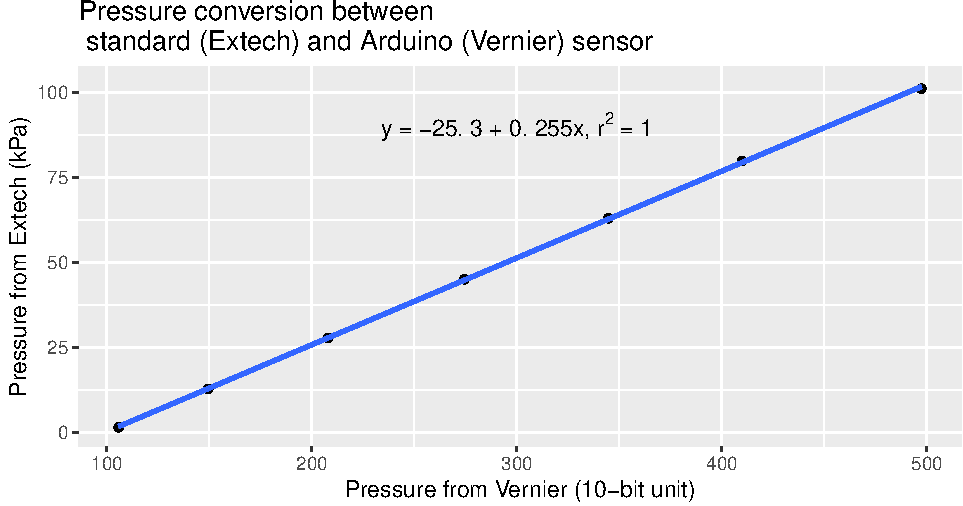
\includegraphics{paper_files/figure-latex/vernier_cal2-1.pdf}

\begin{longtable}[]{@{}rr@{}}
\caption{Varying average pressure readings from Arduino (Vernier)
vs.~Standard (Extech) sensor}\tabularnewline
\toprule
Vernier sensor (10-bit unit) & Extech sensor (kPa)\tabularnewline
\midrule
\endfirsthead
\toprule
Vernier sensor (10-bit unit) & Extech sensor (kPa)\tabularnewline
\midrule
\endhead
105.77 & 1.48\tabularnewline
149.44 & 12.75\tabularnewline
207.92 & 27.79\tabularnewline
274.45 & 45.04\tabularnewline
344.59 & 62.95\tabularnewline
409.80 & 79.86\tabularnewline
497.34 & 101.09\tabularnewline
\bottomrule
\end{longtable}

\subsection{The Adafruit BME280
Sensor}\label{the-adafruit-bme280-sensor}

The Adafruit BME280 sensor, which takes data on temperature, barometric
pressure, and humidity, was calibrated to a Vernier Relative Humidity
Sensor for humidity and the Fieldpiece ST4 Dual Temperature Meter for
temperature. To calibrate for humidity, the BME280 was connected to an
Arduino mega with header pins and programmed to print out data every
second to the serial monitor. The standard for humidity, a Vernier
humidity probe, was connected to the same Arduino board via the Analog
Protoboard Adaptor just like the Vernier Gas Pressure Sensor and also
programmed to print out its humidity readings in the serial monitor
every second. The Vernier Relative Humidity Sensor has a humidity range
of 0\% to 95\%, resolution of 0.16\% RH, operating temperature range of
0 to 85°C, response time of 40 seconds, and total accuracy with its
standard calibration of ±10\% RH. Both sensors were exposed to
environments with various humidity levels: the Menlo Quad at 3:00 PM and
a shower 30, 60, 90, and 120 seconds after turning the hot water on.
Multiple consecutive relative humidity readings from both sensors at
each time point were then manually recorded in a csv file. Graph 8,
shown below, depicts the relative humidity conversion between the output
of the standard (Vernier) sensor and that of the Arduino (BME280) sensor
across various humidity levels.

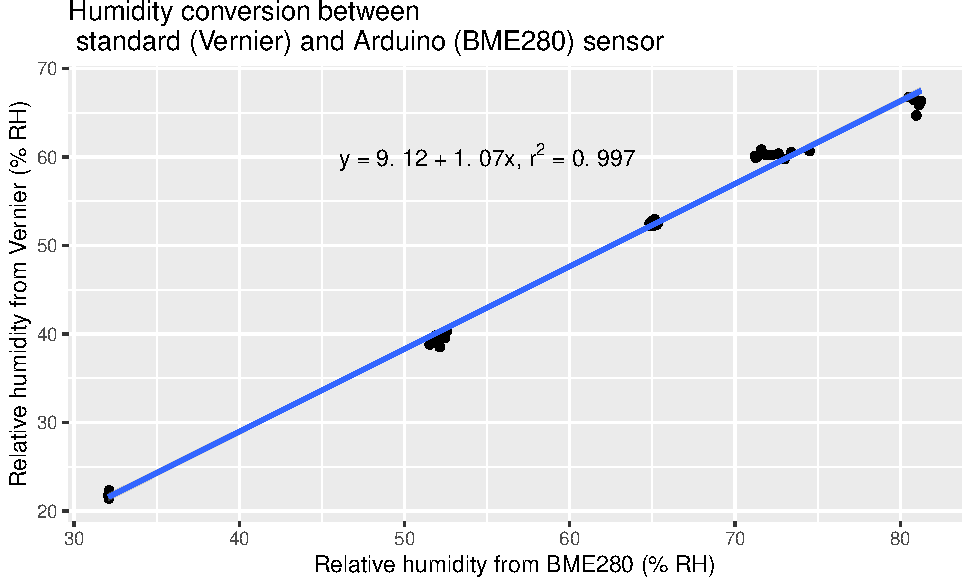
\includegraphics{paper_files/figure-latex/bme-1.pdf}

In order to calibrate the temperature readings of the BME280 to a
standard, the Fieldpiece ST4 Dual Temperature Meter, both sensors were
placed in multiple locations of varying temperatures: a freezer,
refrigerator, and the Menlo Quad at two different times of the day.

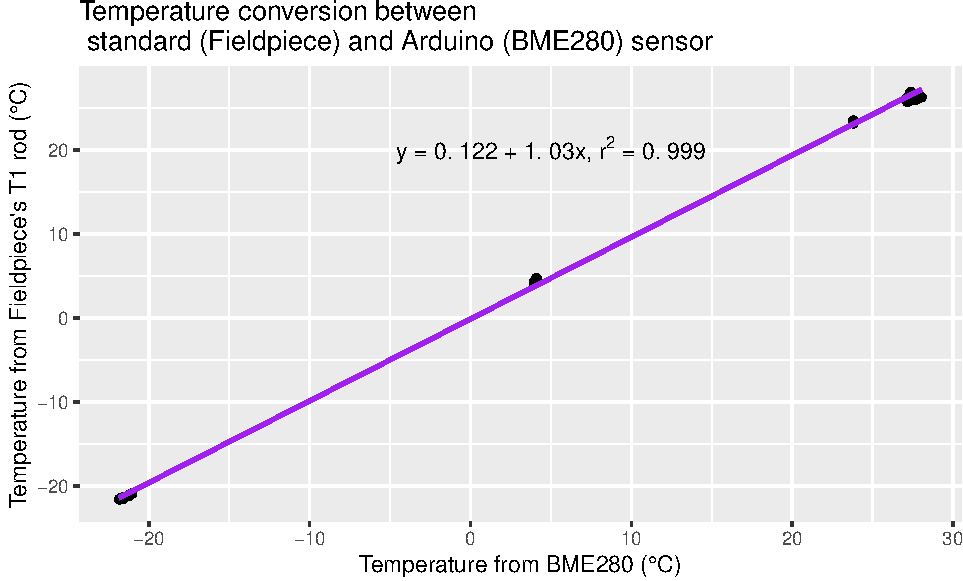
\includegraphics{paper_files/figure-latex/bme_temp-1.pdf}

\begin{longtable}[]{@{}lr@{}}
\caption{Percent errors for the group sensors used relative to
standards}\tabularnewline
\toprule
Experiments & Percent error (\%)\tabularnewline
\midrule
\endfirsthead
\toprule
Experiments & Percent error (\%)\tabularnewline
\midrule
\endhead
Pressure & 0.459\tabularnewline
Humidity & 0.659\tabularnewline
Temperature & 0.429\tabularnewline
\bottomrule
\end{longtable}

\section{Experimental Results}\label{experimental-results}

lorem ipsum

\section{Conclusion}\label{conclusion}

lorem ipsum


\end{document}
